\section{Messwerttabellen}

\label{sec:messtabellen}

\begin{figure}[H]
	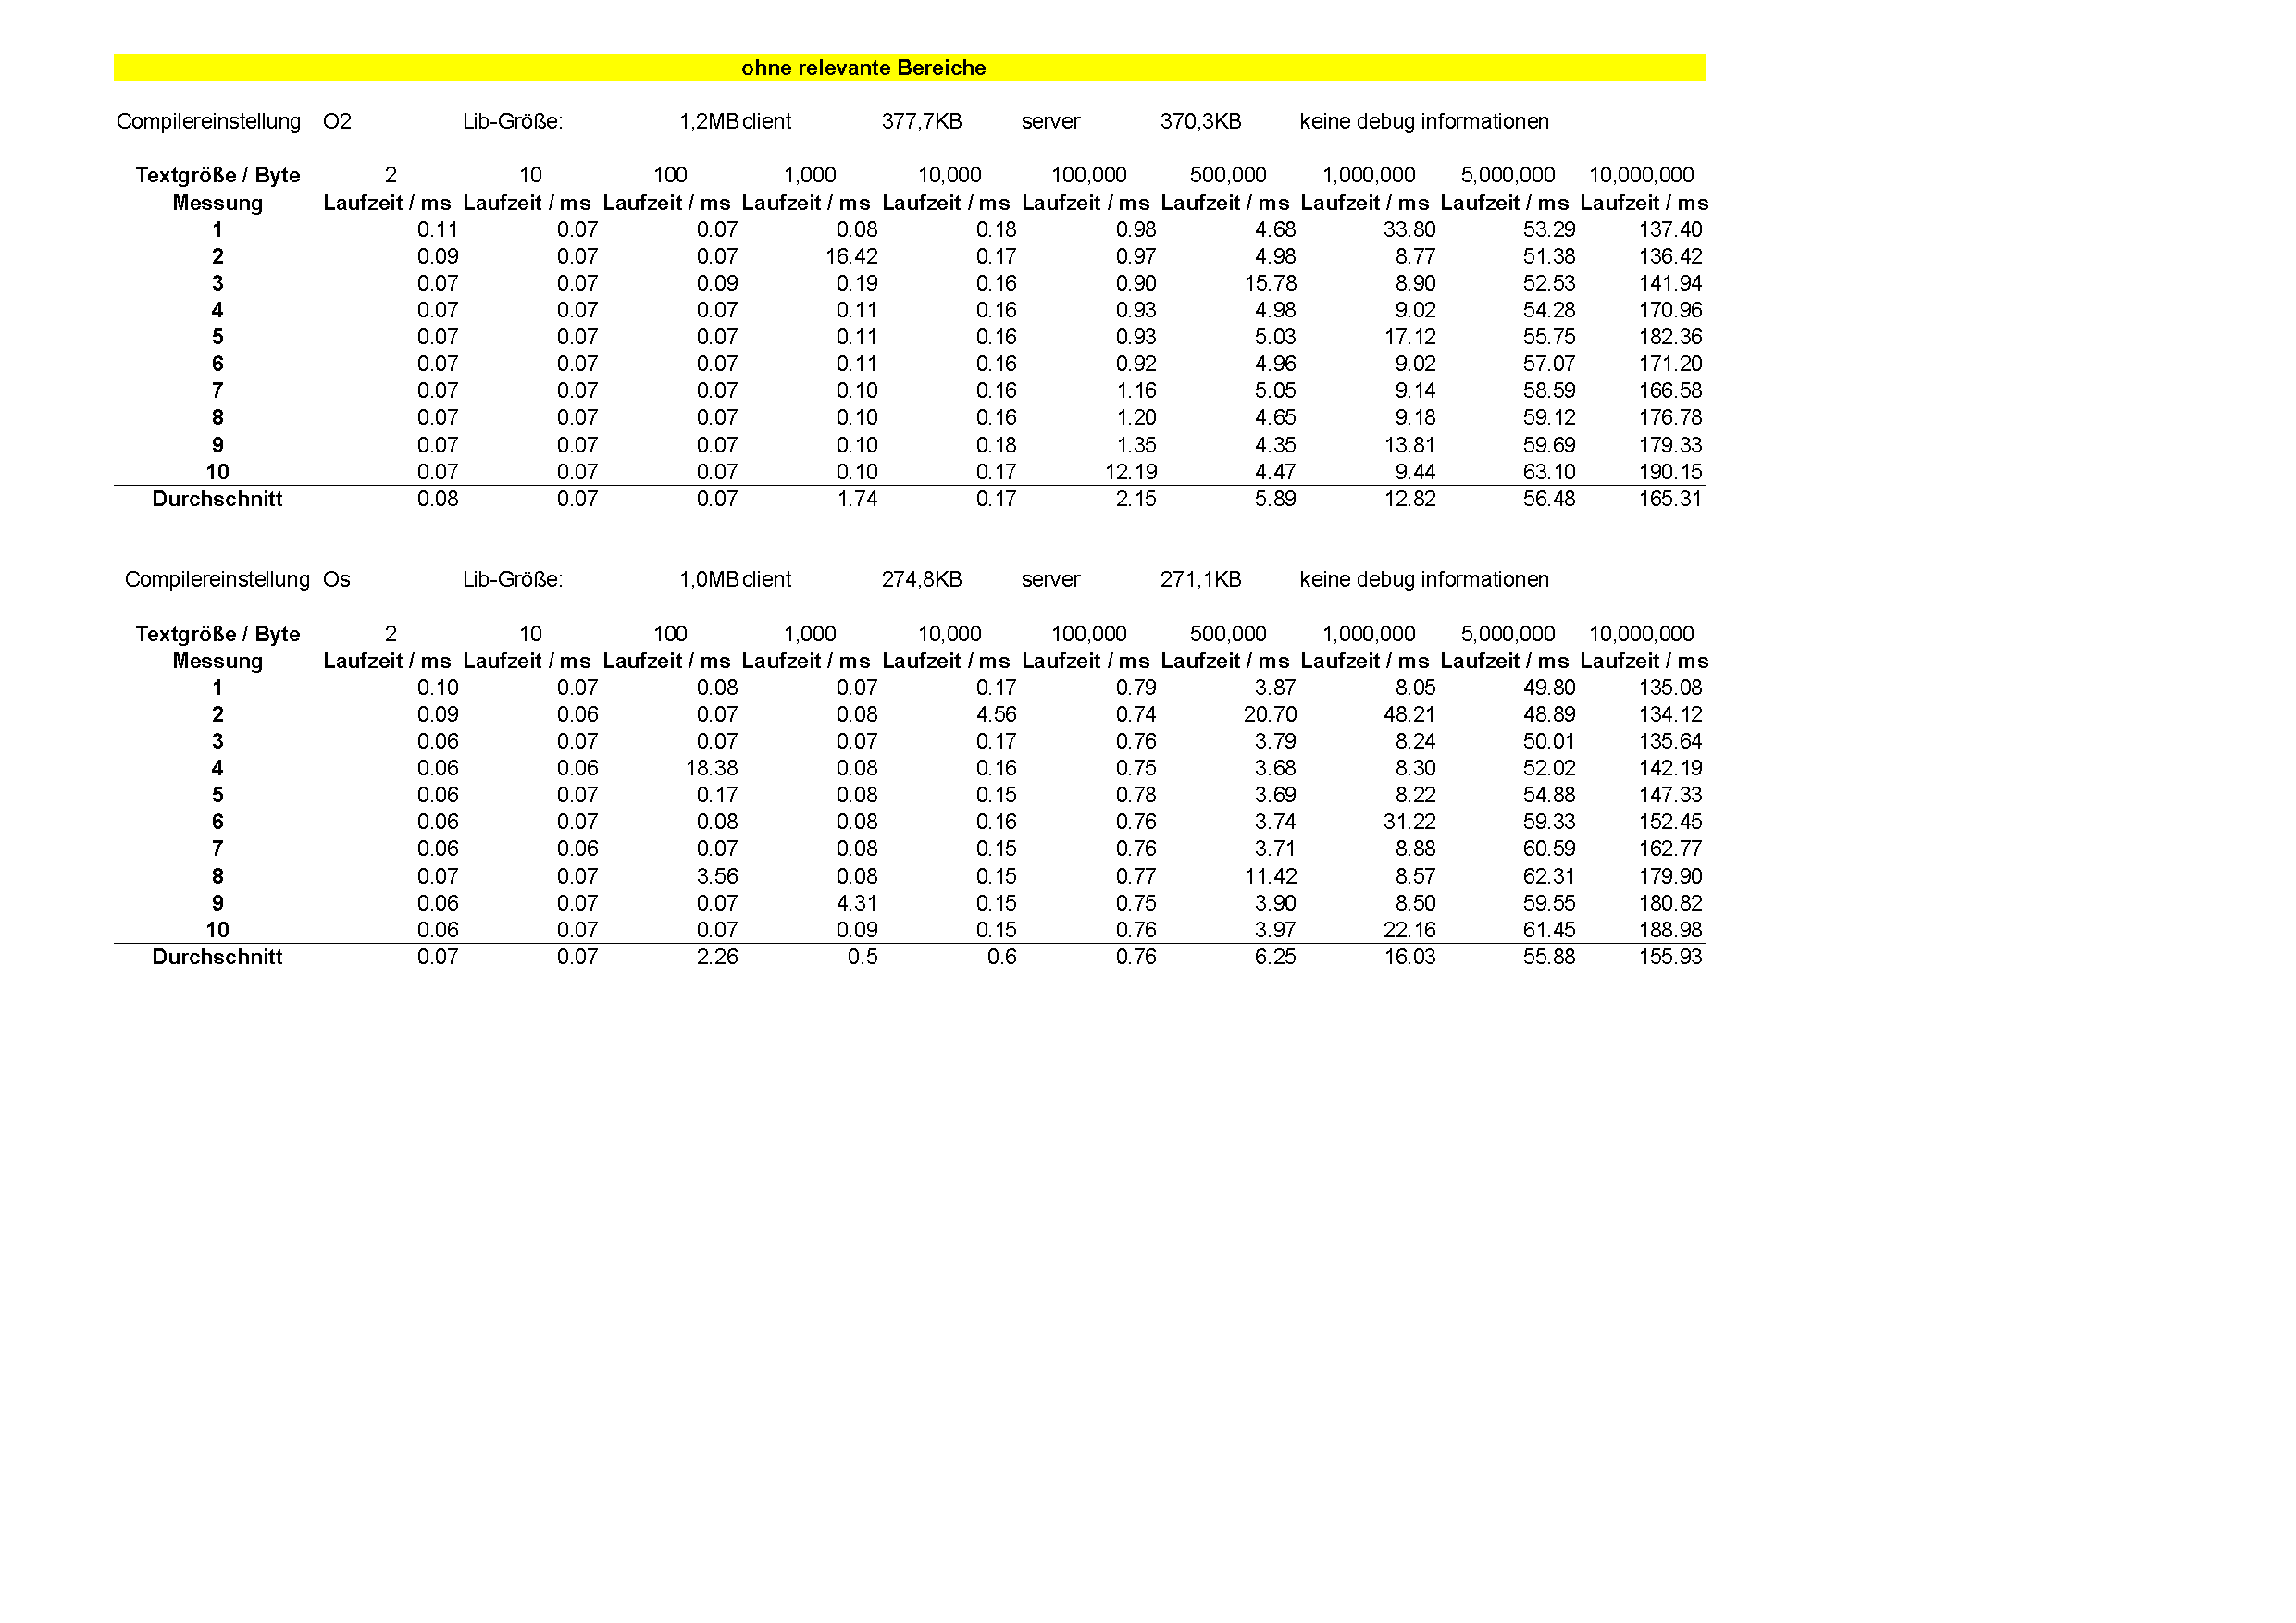
\includegraphics[angle=90,scale=.5]{MessungNormal_worp.pdf}
	\caption{Messung-Normal}	
\end{figure}

\newpage

\begin{figure}[H]
	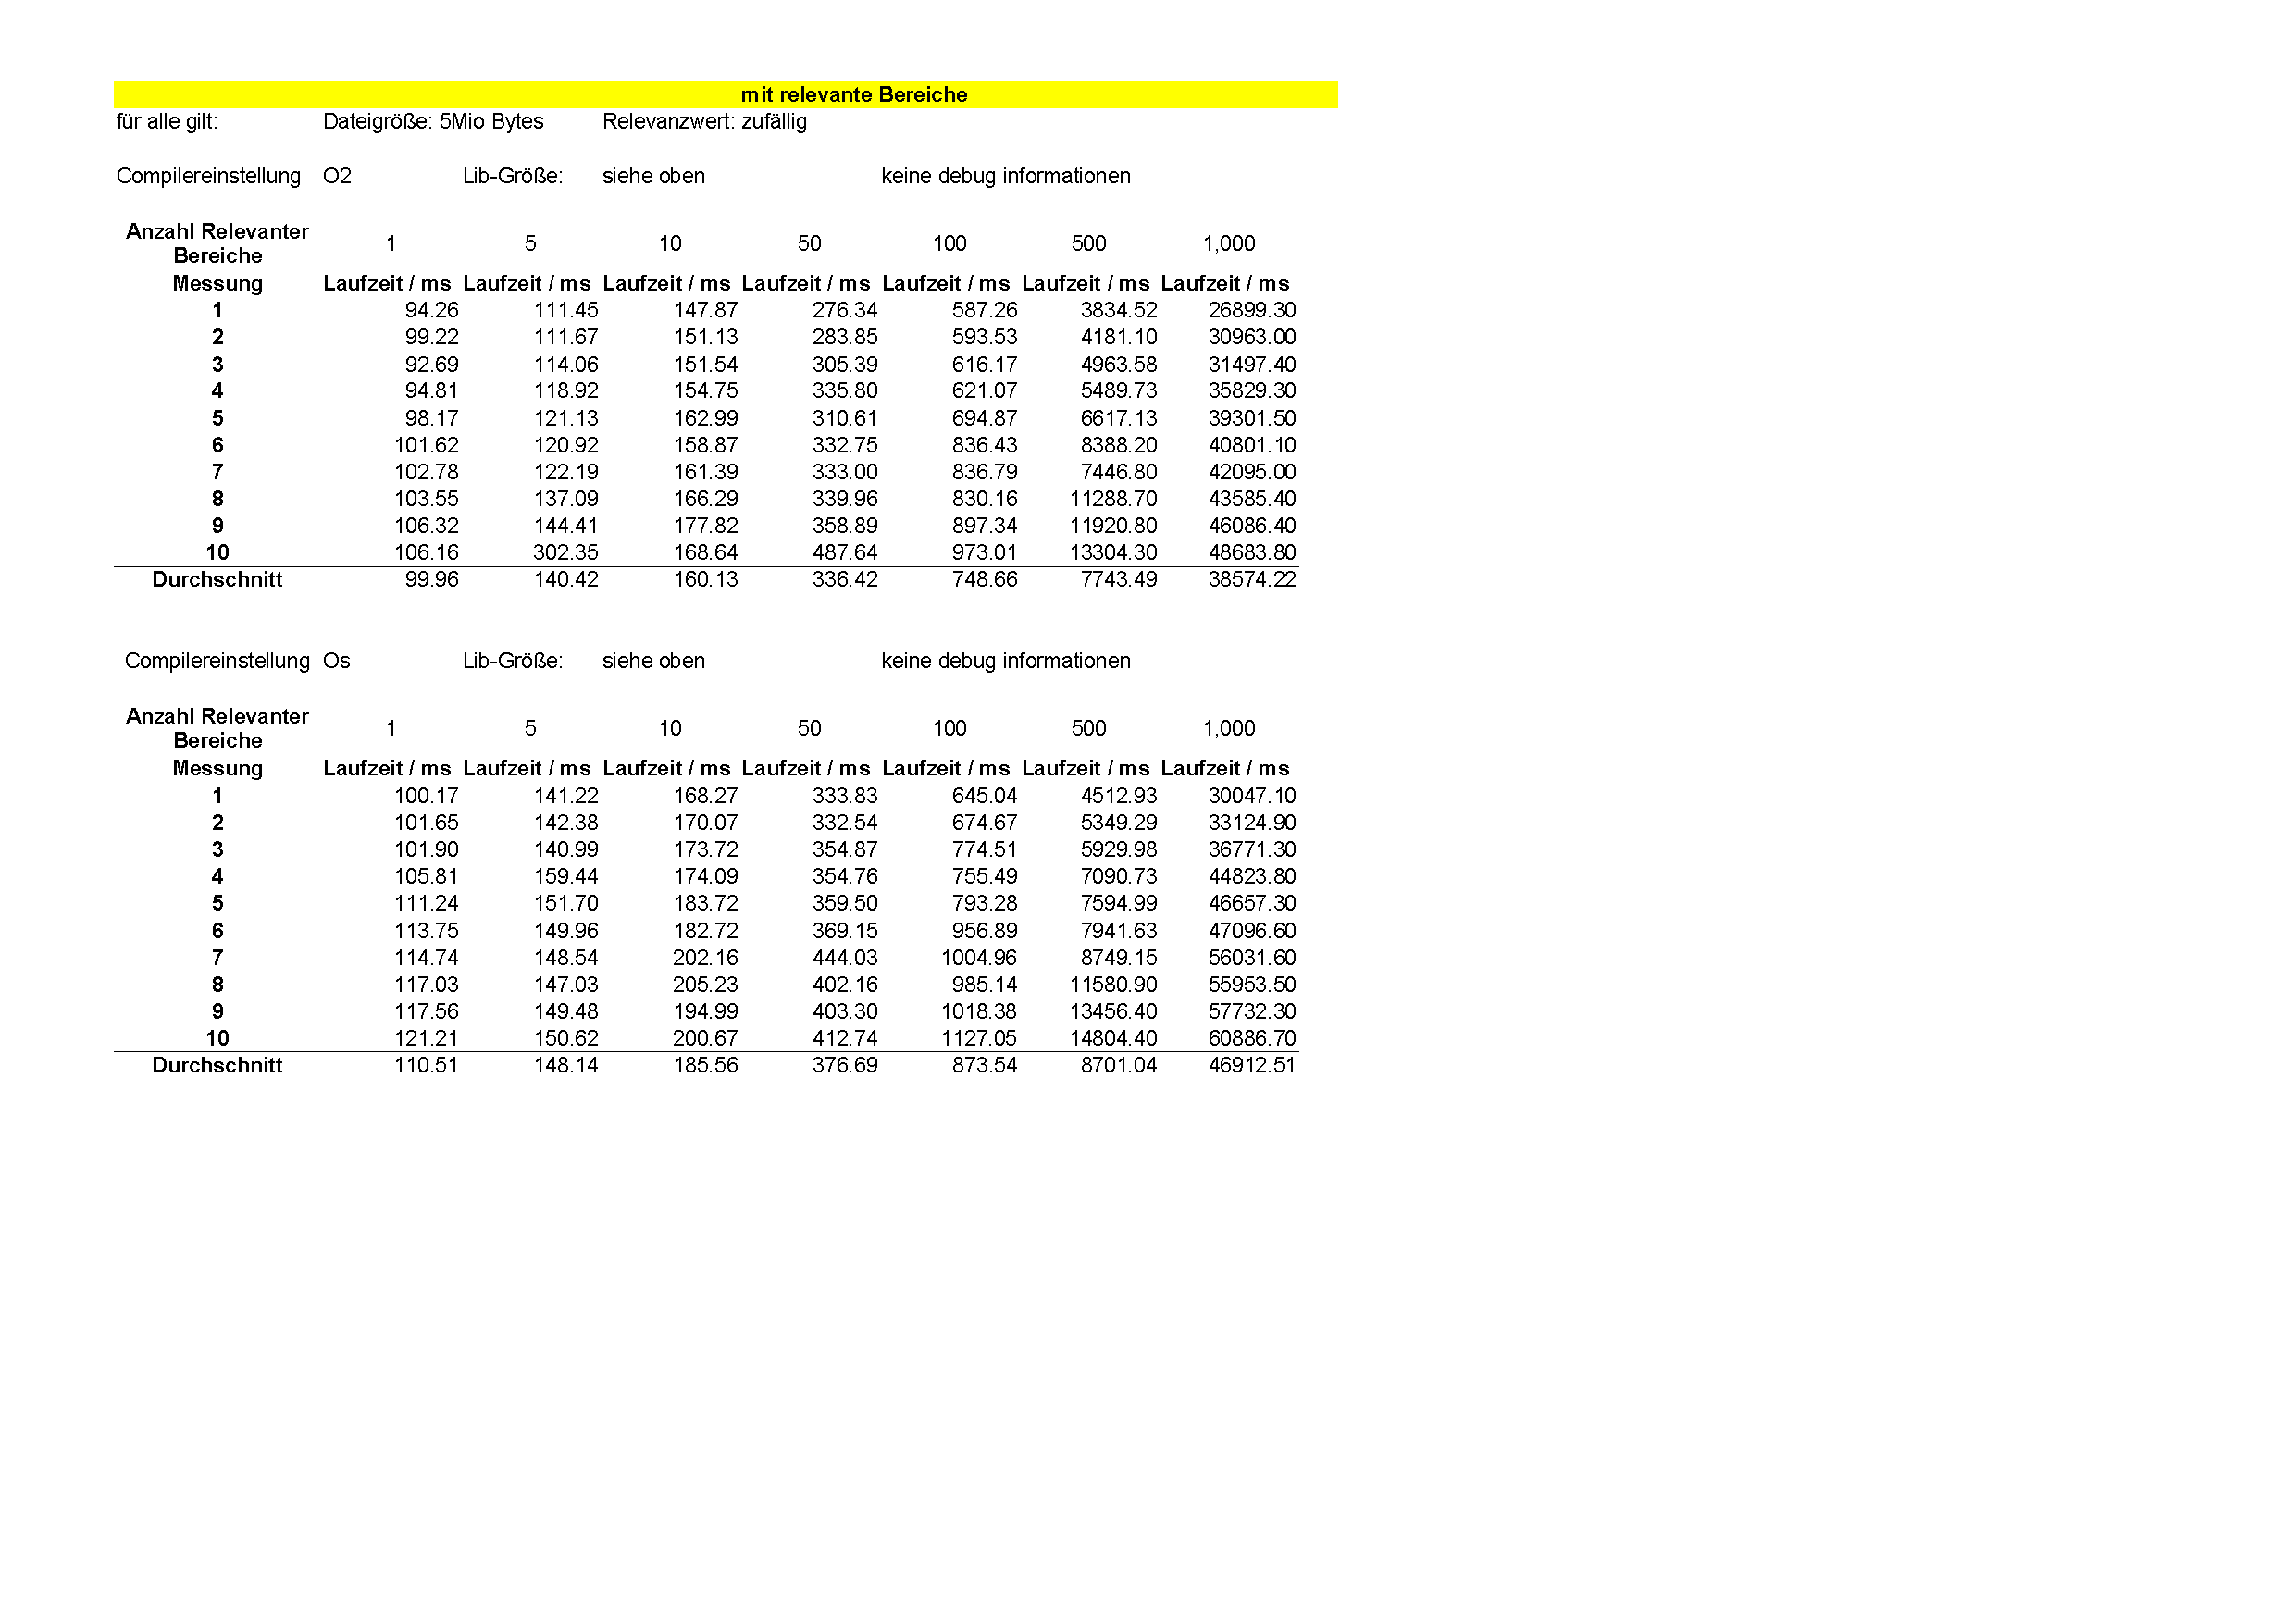
\includegraphics[angle=90,scale=.7]{MessungNormal_wrp.pdf}
	\caption{Messung-Normal}	
\end{figure}

\newpage

\begin{figure}[H]
	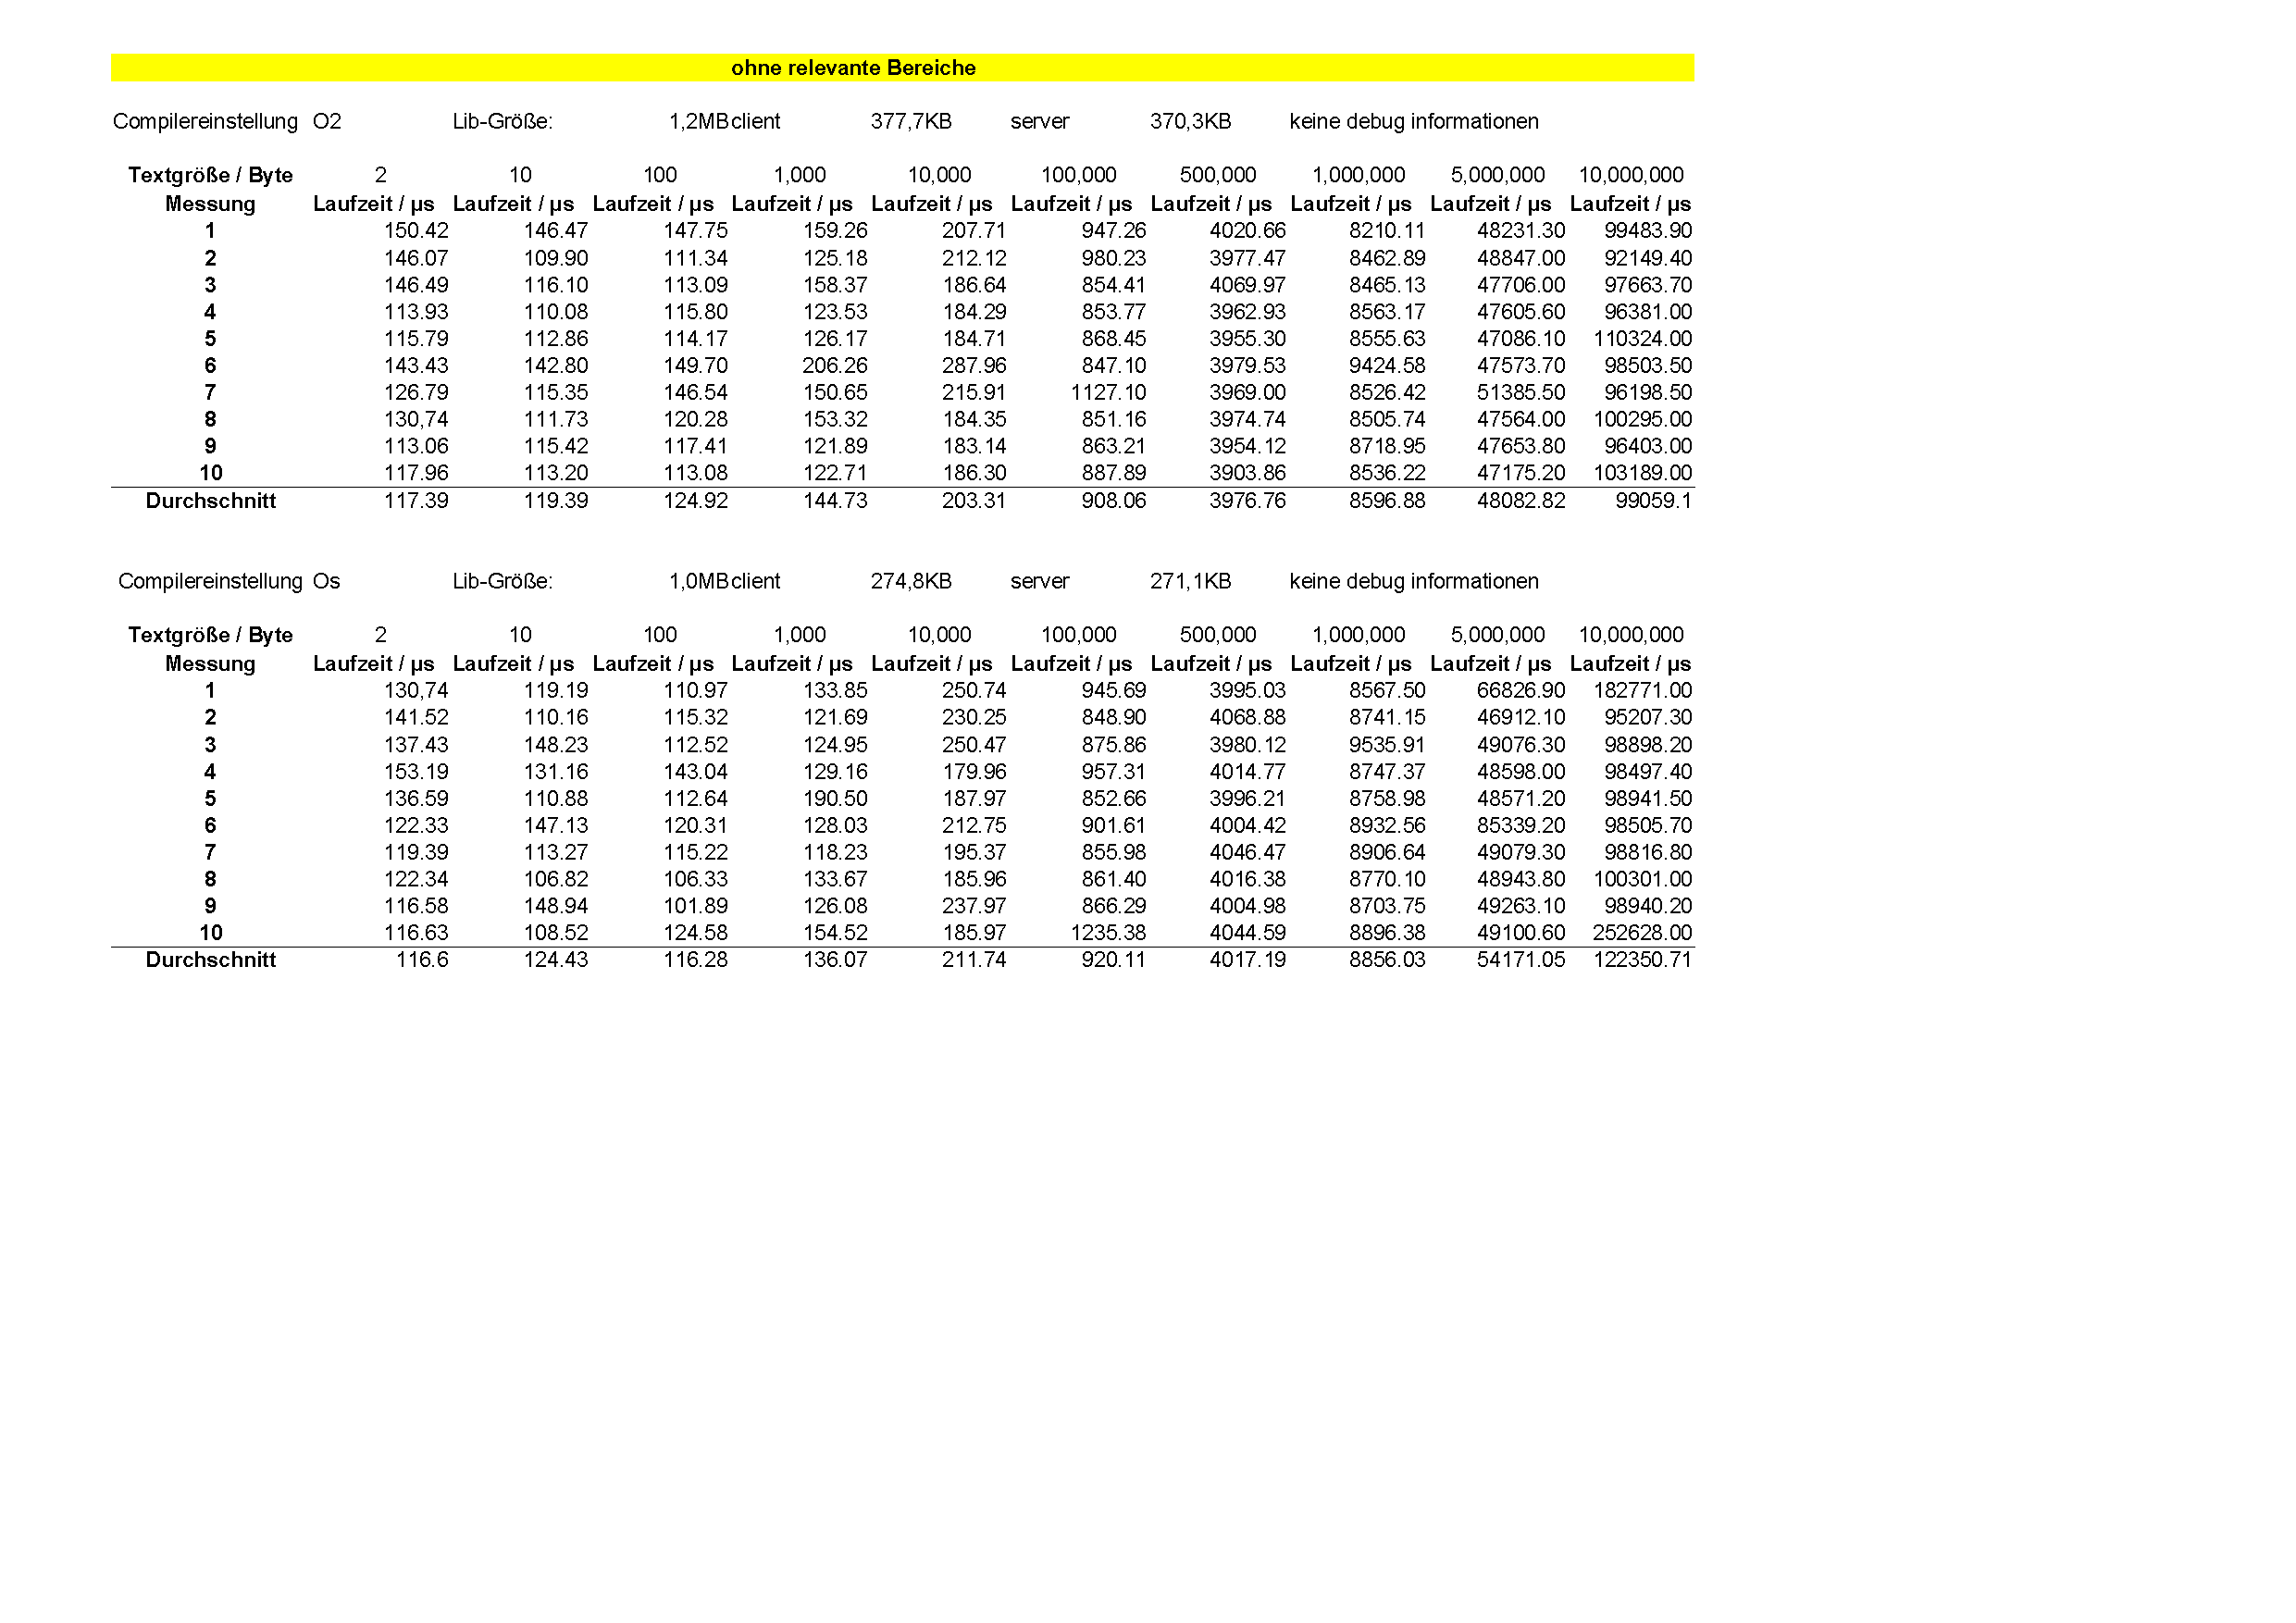
\includegraphics[angle=90,scale=.75]{MessungInitial_worp.pdf}
	\caption{Messung-Initial}	
\end{figure}

\newpage

\begin{figure}[H]
	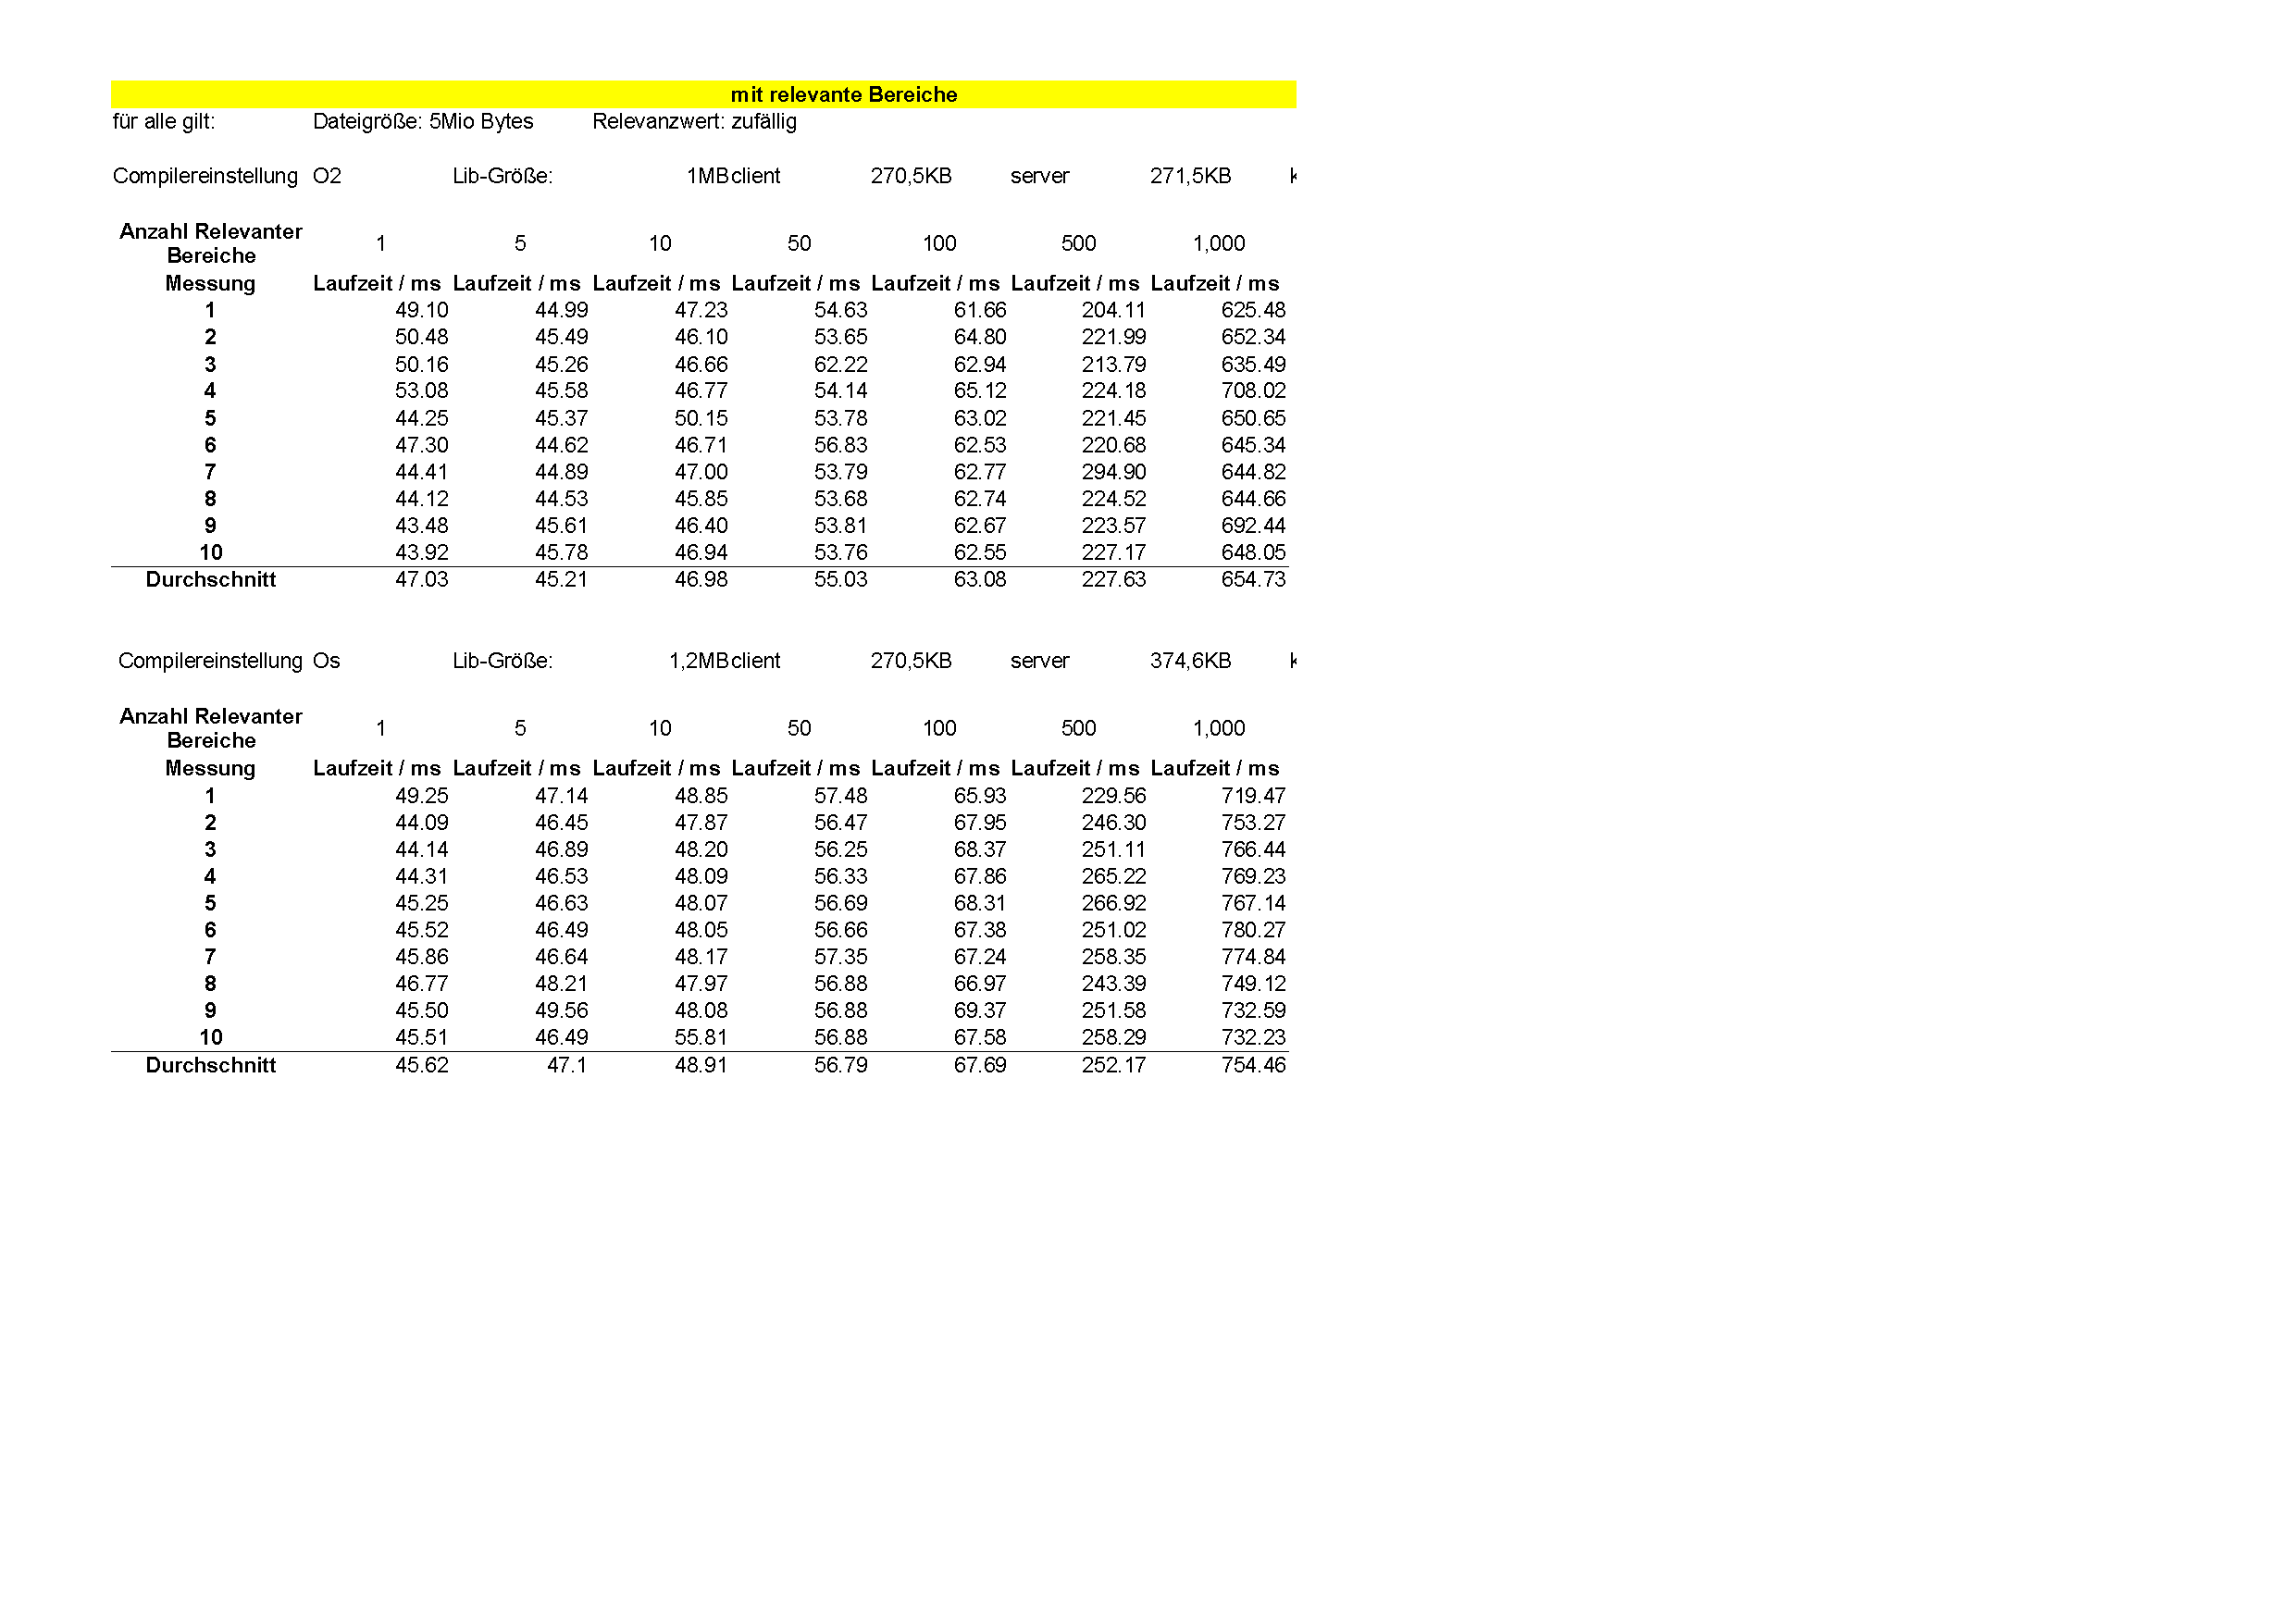
\includegraphics[angle=90,scale=.75]{MessungInitial_wrp.pdf}
	\caption{Messung-Initial}	
\end{figure}

% Die restlichen Diagramme. Müssen eventuell noch angepasst werden.
\section{Diagramme}
\label{sec:Diagramme}

\begin{figure}[H]
	\centering
	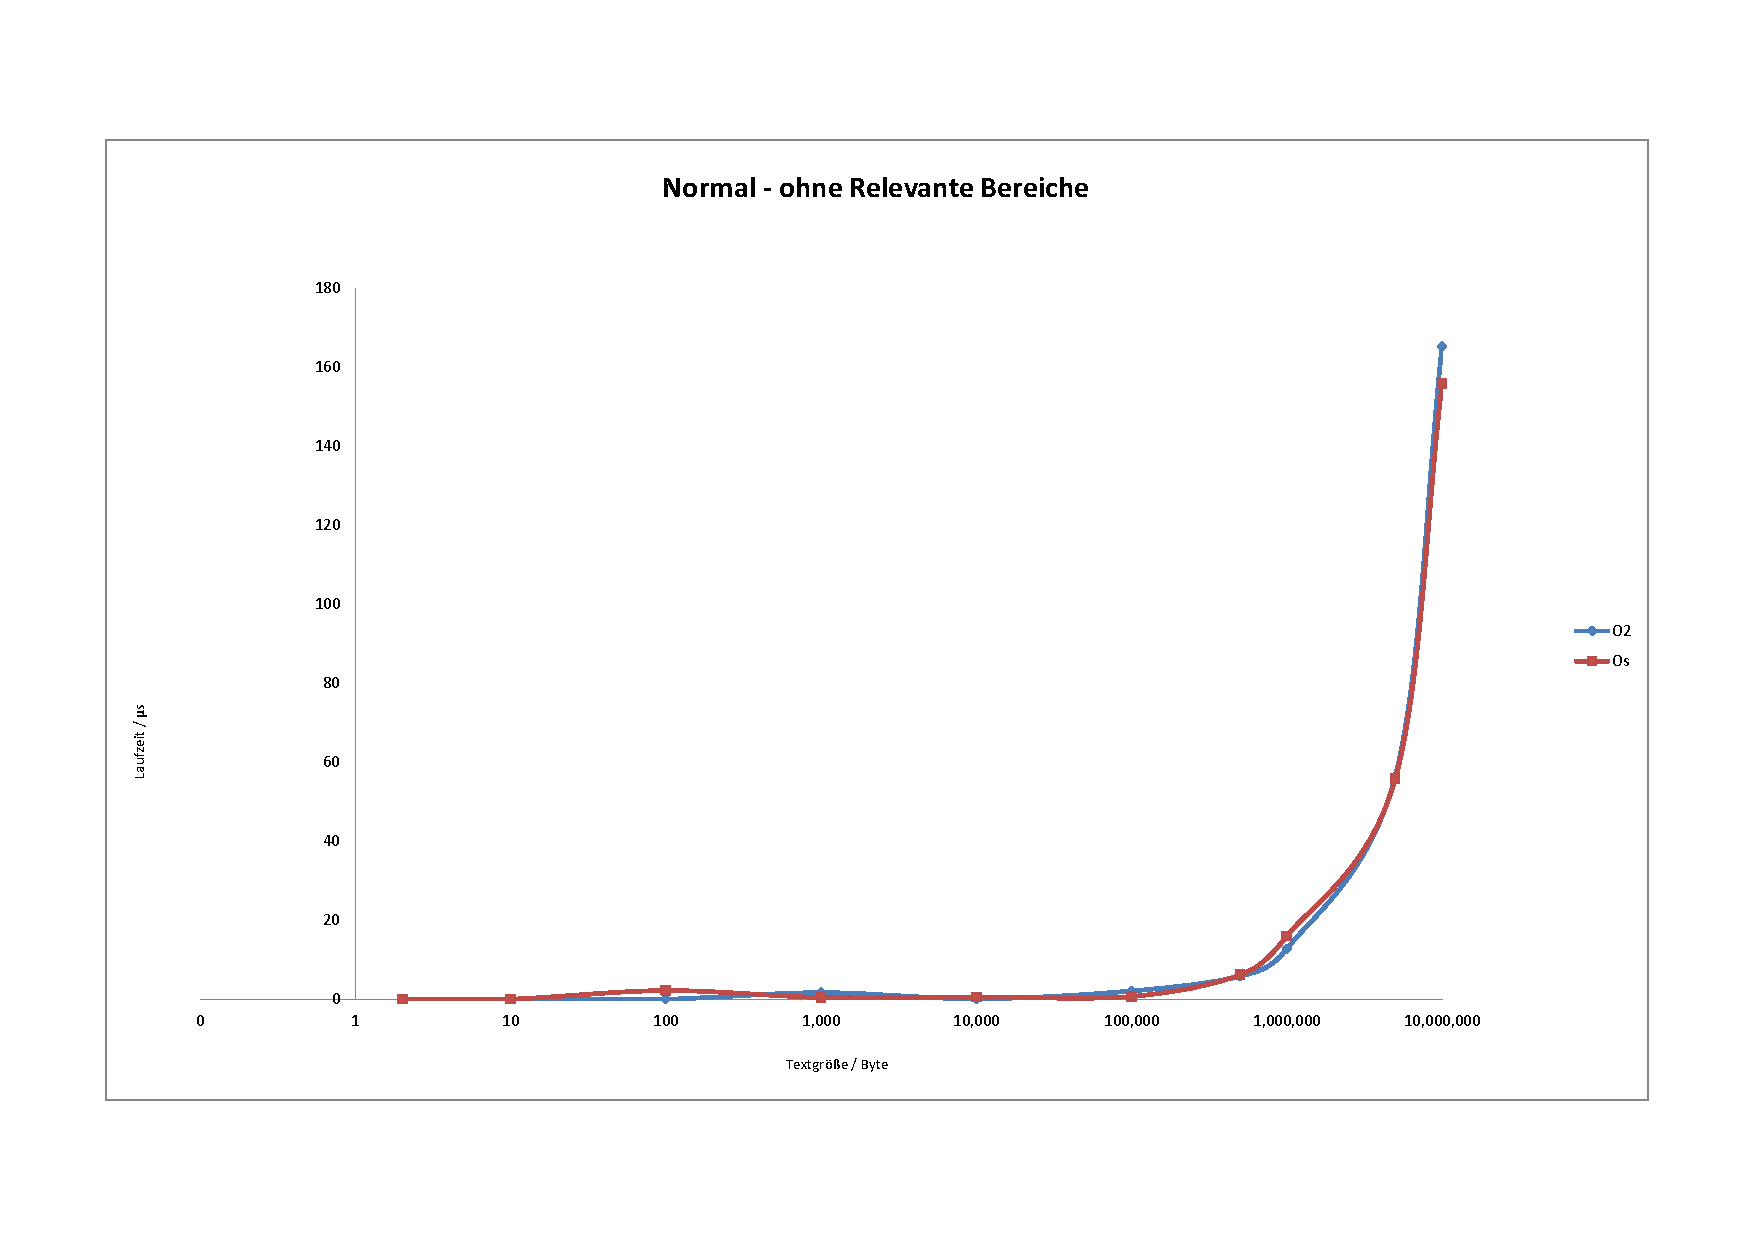
\includegraphics[angle=90,scale=.8]{DiagrammNormal_worp.pdf}
	\label{fig:diagrammNormal_worp}
	\caption{Messung-Normal ohne relevante Bereiche}
\end{figure}

\begin{figure}[H]
	\centering
	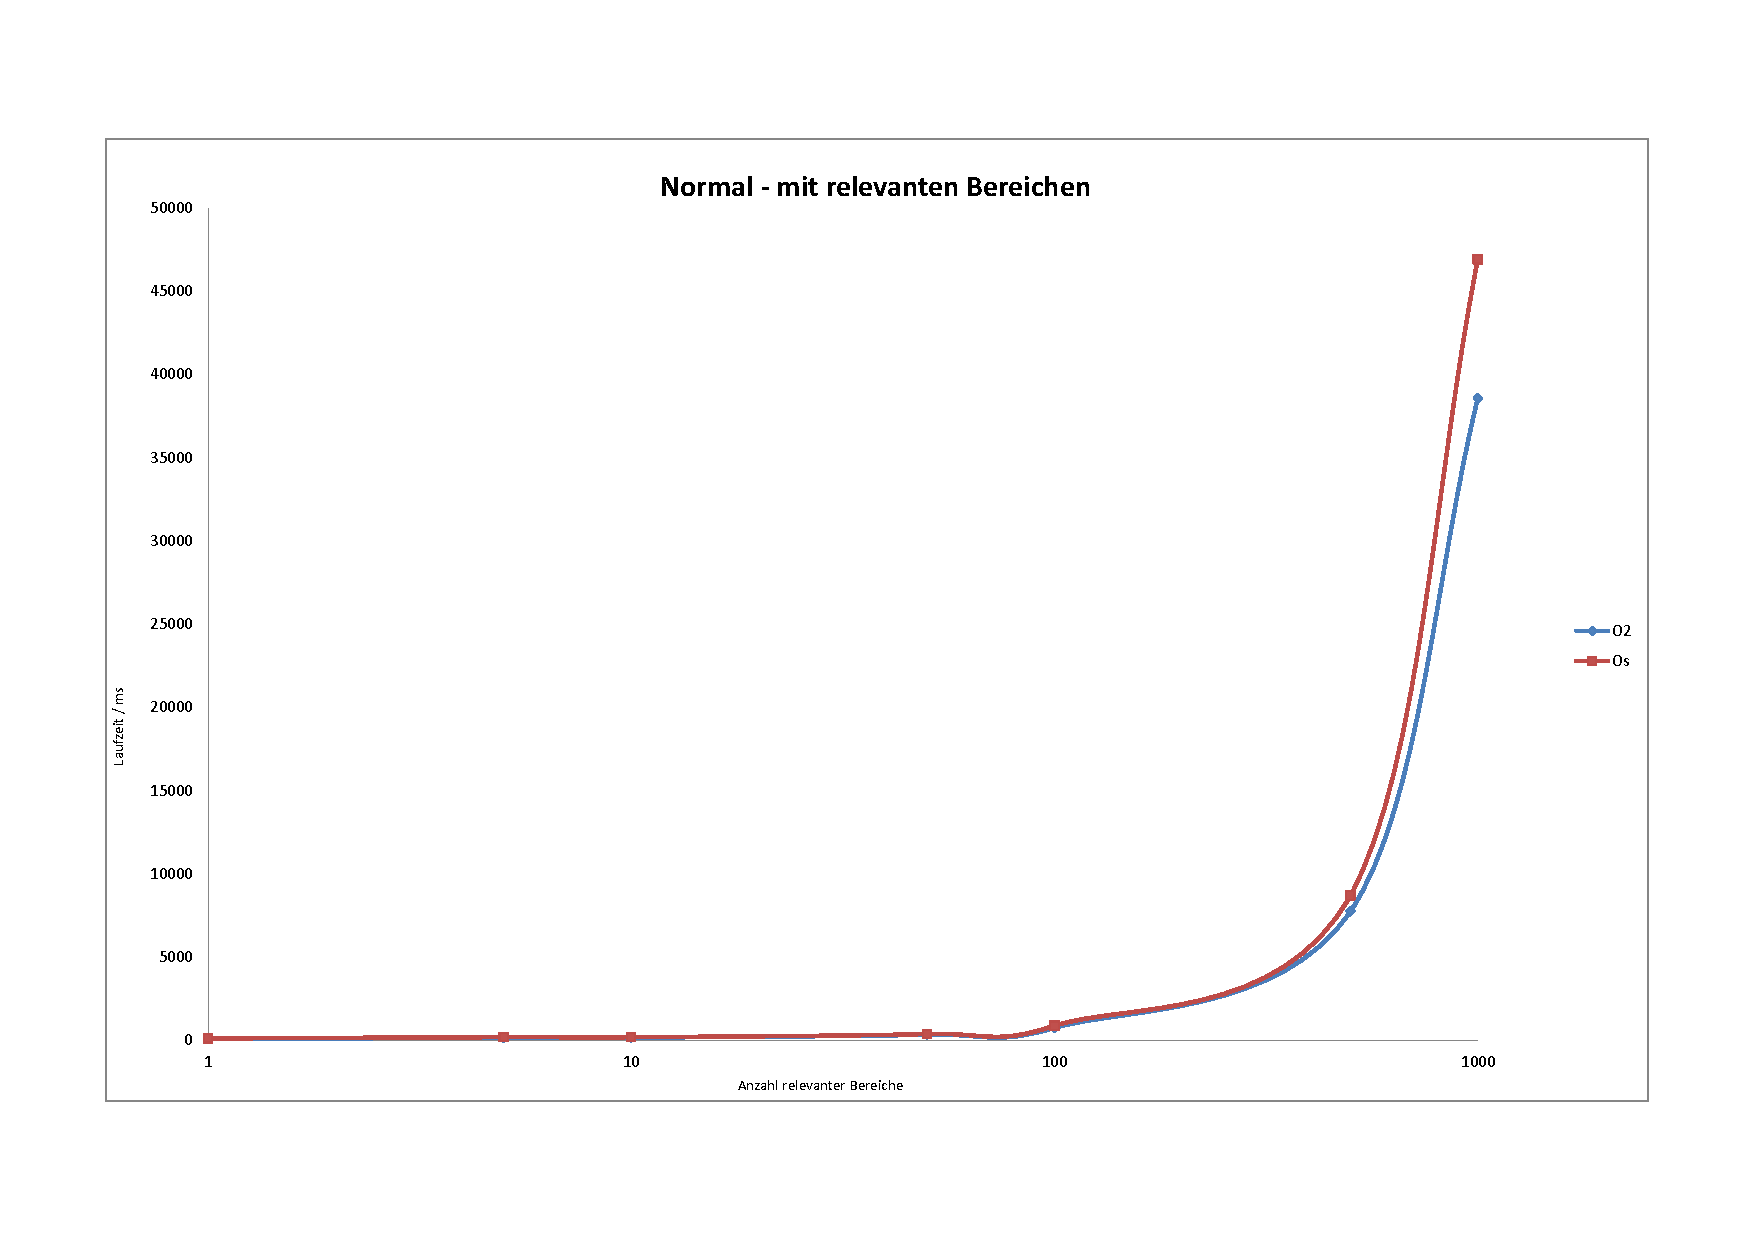
\includegraphics[angle=90,scale=.8]{DiagrammNormal_wrp.pdf}
	\label{fig:diagrammNormal_wrp}
	\caption{Messung-Normal mit relevanten Bereichen}
\end{figure}

% Größere Darstellung der Datenaufsplittung
\section{Datenaufschlüsselung}
\label{sec:Datenaufschluesselung}

\begin{figure}[H]
	\centering
	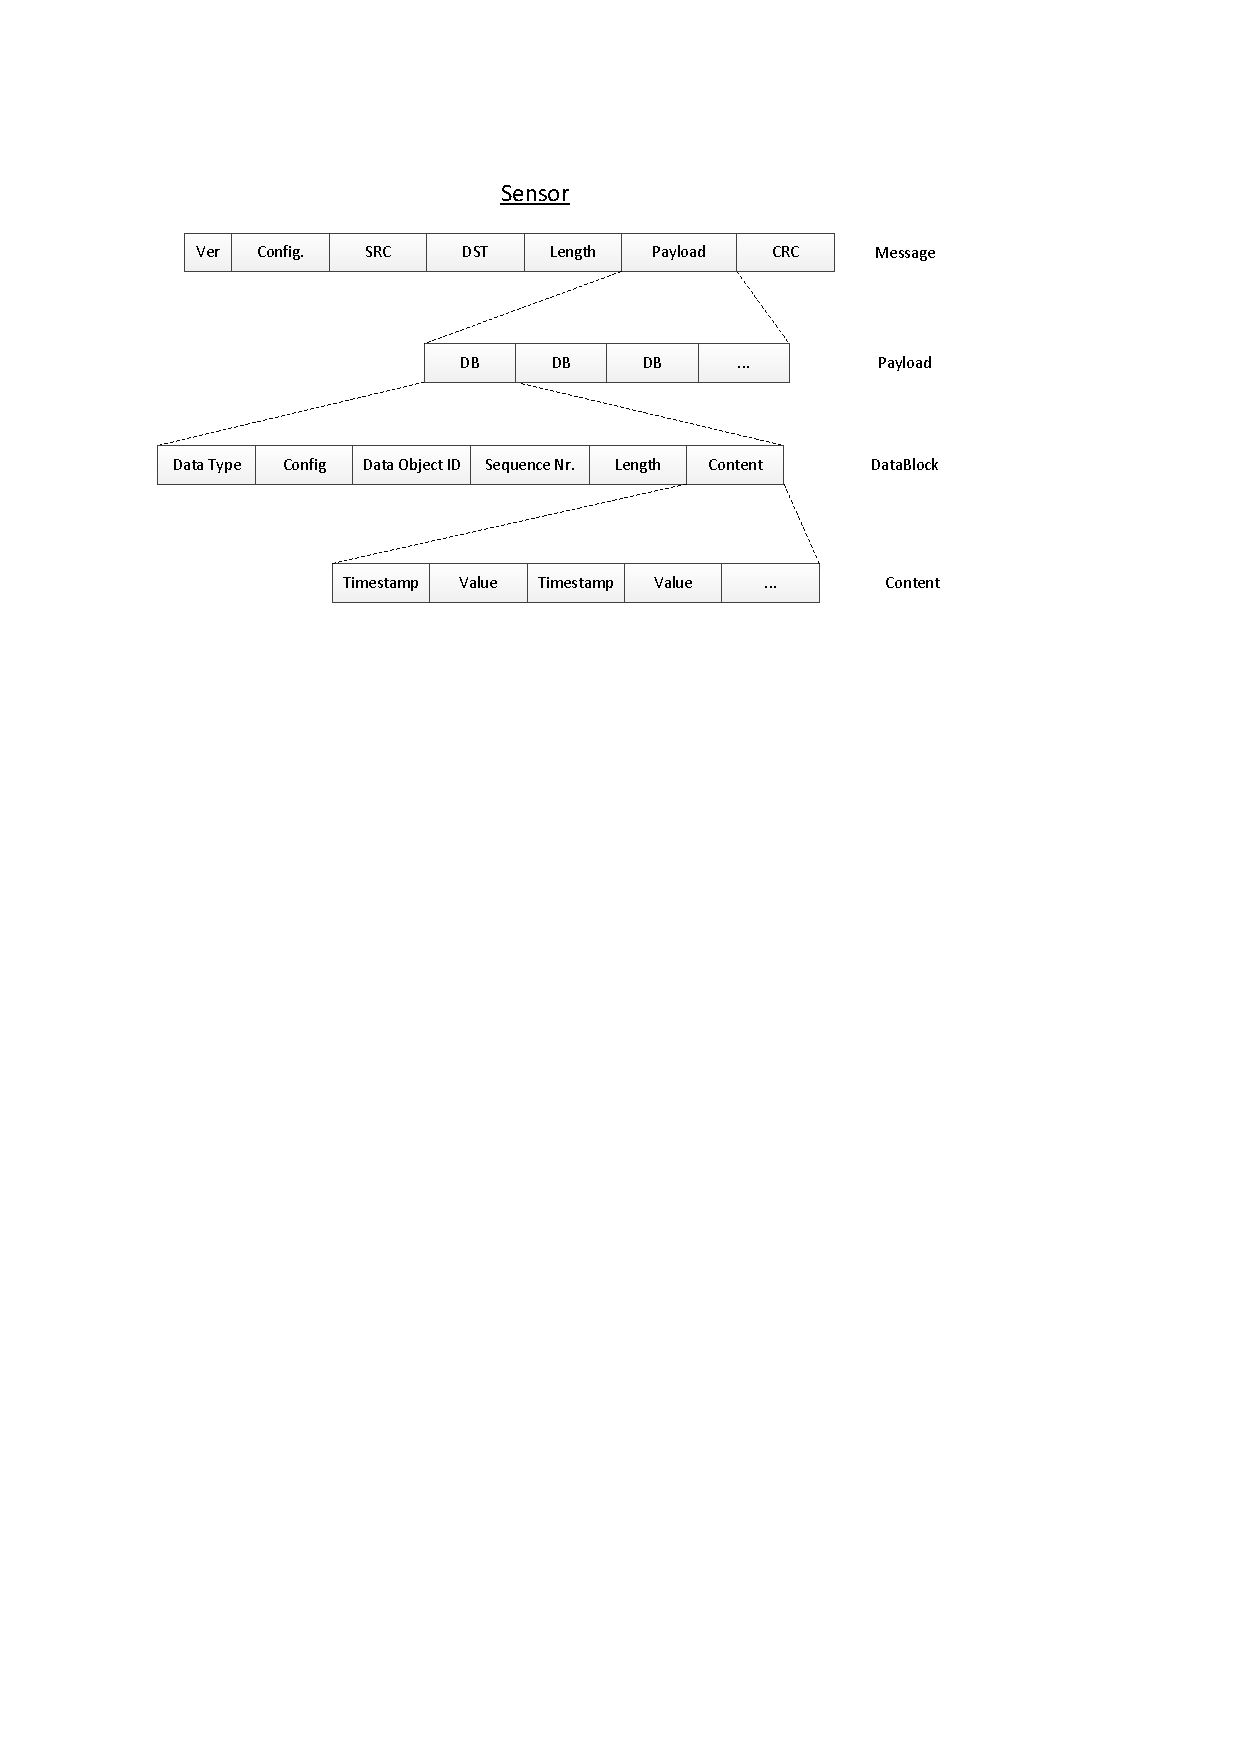
\includegraphics{DatenaufschluesselungSensor.pdf}
	\caption{Datenaufschlüsselung-Sensor}
\end{figure}

\begin{figure}[H]
	\centering
	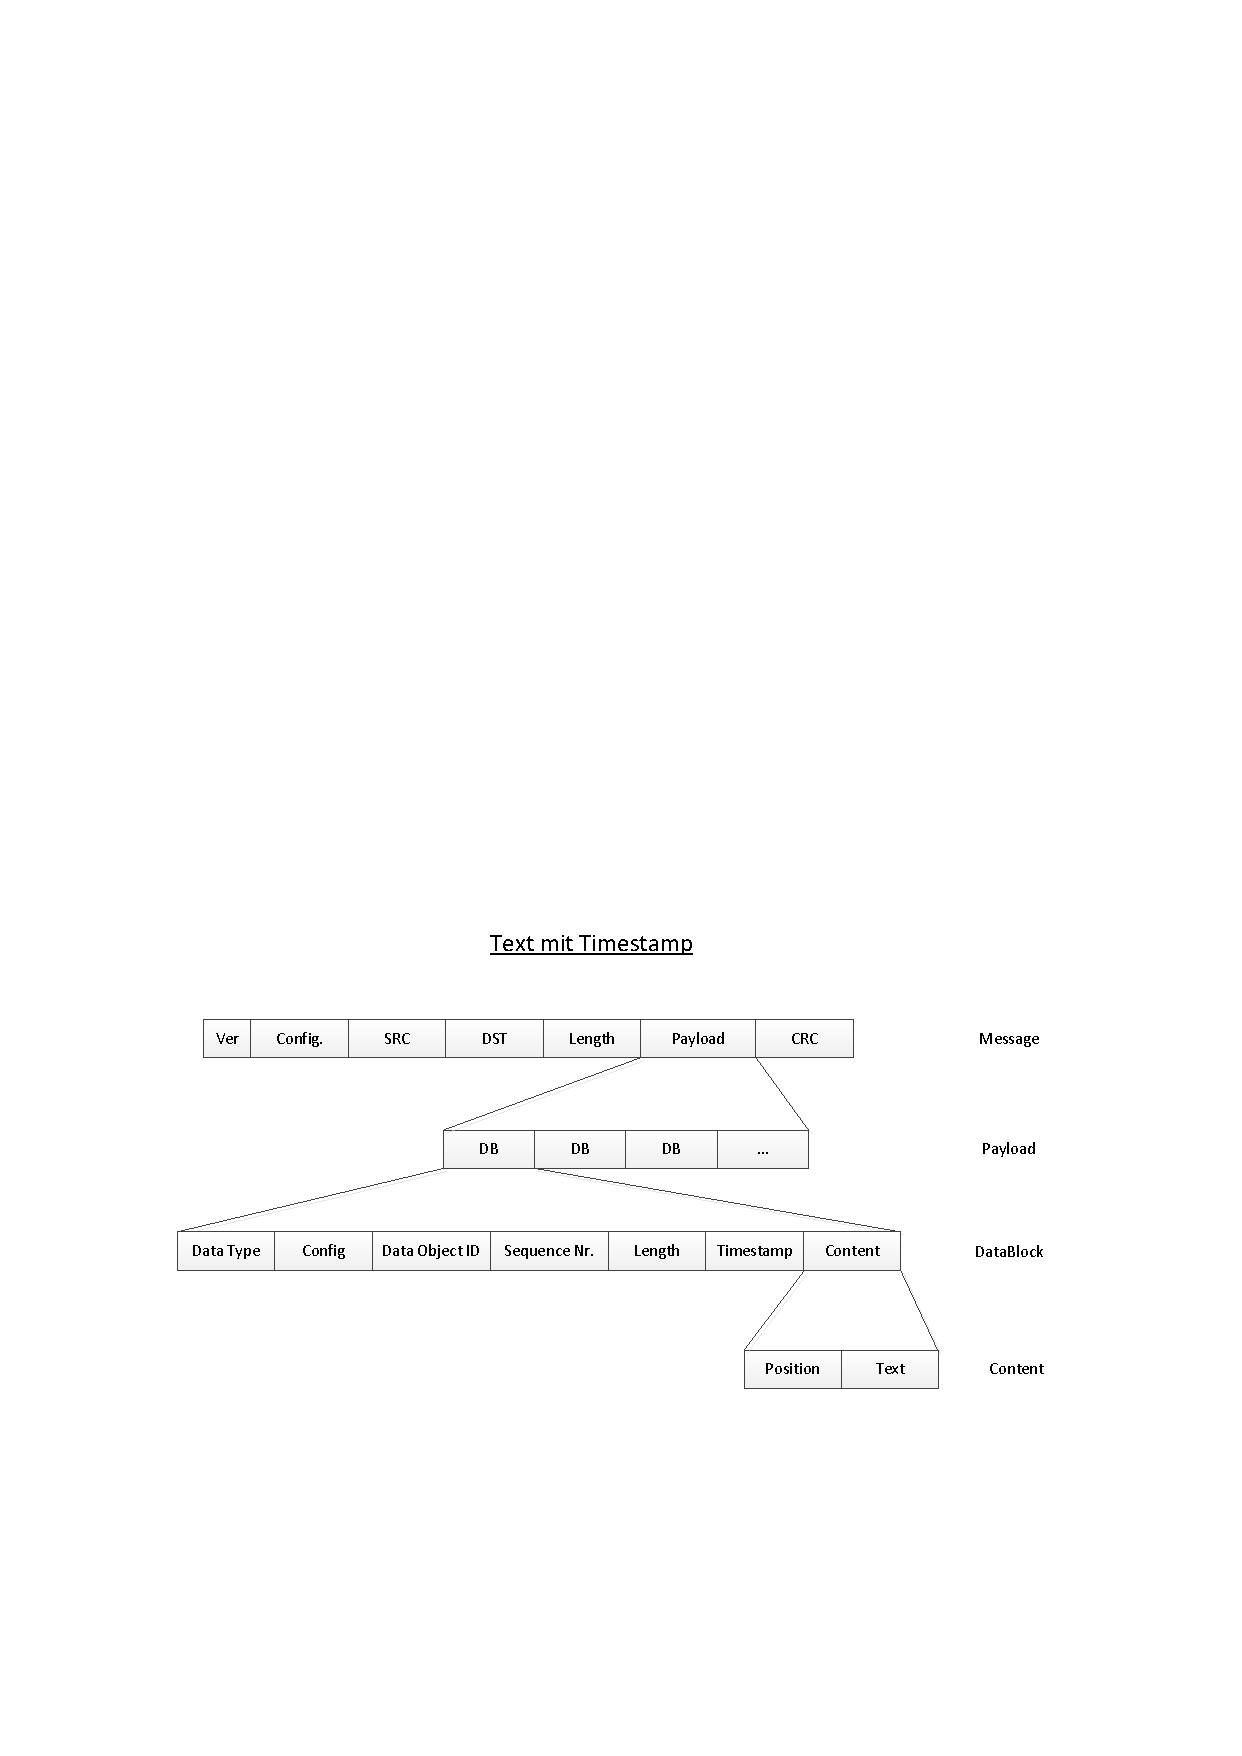
\includegraphics{DatenaufschluesselungText.pdf}
	\caption{Datenaufschlüsselung-Text}
\end{figure}
